% 07_cross_outcome.tex
% Section 7: Cross-Outcome Analysis

\chapter{Cross-Outcome Analysis}
\label{sec:cross-outcome}

Each NBA game on Polymarket features two outcomes: home team wins and away team wins. This section examines the relationship between these paired outcomes, including price complementarity (do probabilities sum to 1?), arbitrage opportunities, and depth asymmetries between outcomes.

%------------------------------------------------------------------------------
% 7.1 Binary Market Theory
%------------------------------------------------------------------------------
\section{Binary Market Theory}

In a binary market with two mutually exclusive, collectively exhaustive outcomes, basic probability theory requires that outcome probabilities sum to exactly 1. If the home team has a 60\% win probability, the away team must have a 40\% win probability by definition.

In prediction markets, prices represent these probabilities. Therefore, in an efficient binary market:

\begin{equation}
P_{\text{Home}} + P_{\text{Away}} = 1.00
\end{equation}

Deviations from this condition create potential arbitrage opportunities:

\textbf{Sum $<$ 1 (Underpricing):} If prices sum to less than 1 (e.g., Home = 0.55, Away = 0.43, sum = 0.98), a trader can buy both outcomes for \$0.98 total and receive \$1.00 at resolution regardless of which team wins---a guaranteed 2\% profit.

\textbf{Sum $>$ 1 (Overpricing/Overround):} If prices sum to more than 1 (e.g., Home = 0.56, Away = 0.46, sum = 1.02), market makers extract a 2\% ``vigorish'' or overround. In traditional sports betting, this overround represents the bookmaker's profit margin.

\begin{methodbox}[Arbitrage in Binary Markets]
\textbf{Arbitrage} exploits price discrepancies to guarantee risk-free profit.

\textbf{Binary Market Arbitrage:} In a market with outcomes A and B:
\begin{equation}
\text{Arbitrage Profit} = 1 - (P_A + P_B)
\end{equation}

If $P_A + P_B < 1$: Buy both outcomes for guaranteed profit of $(1 - P_A - P_B)$.

\textbf{Example:} Home = \$0.52, Away = \$0.46, Sum = \$0.98
\begin{itemize}
    \item Buy 1 Home contract: \$0.52
    \item Buy 1 Away contract: \$0.46
    \item Total cost: \$0.98
    \item Payout (either outcome): \$1.00
    \item Guaranteed profit: \$0.02 (2.0\% return)
\end{itemize}

\textbf{Practical Constraints:} Transaction costs, capital requirements, and execution risk mean that small deviations (under 2--3\%) may not be profitably arbitraged.
\end{methodbox}

%------------------------------------------------------------------------------
% 7.2 Probability Sum Analysis
%------------------------------------------------------------------------------
\section{Probability Sum Analysis}

Figure~\ref{fig:arbitrage} presents the distribution of probability sums (Home + Away) across our sample. This analysis uses mid-prices to assess the theoretical sum at each point in time.

\begin{figure}[H]
\centering
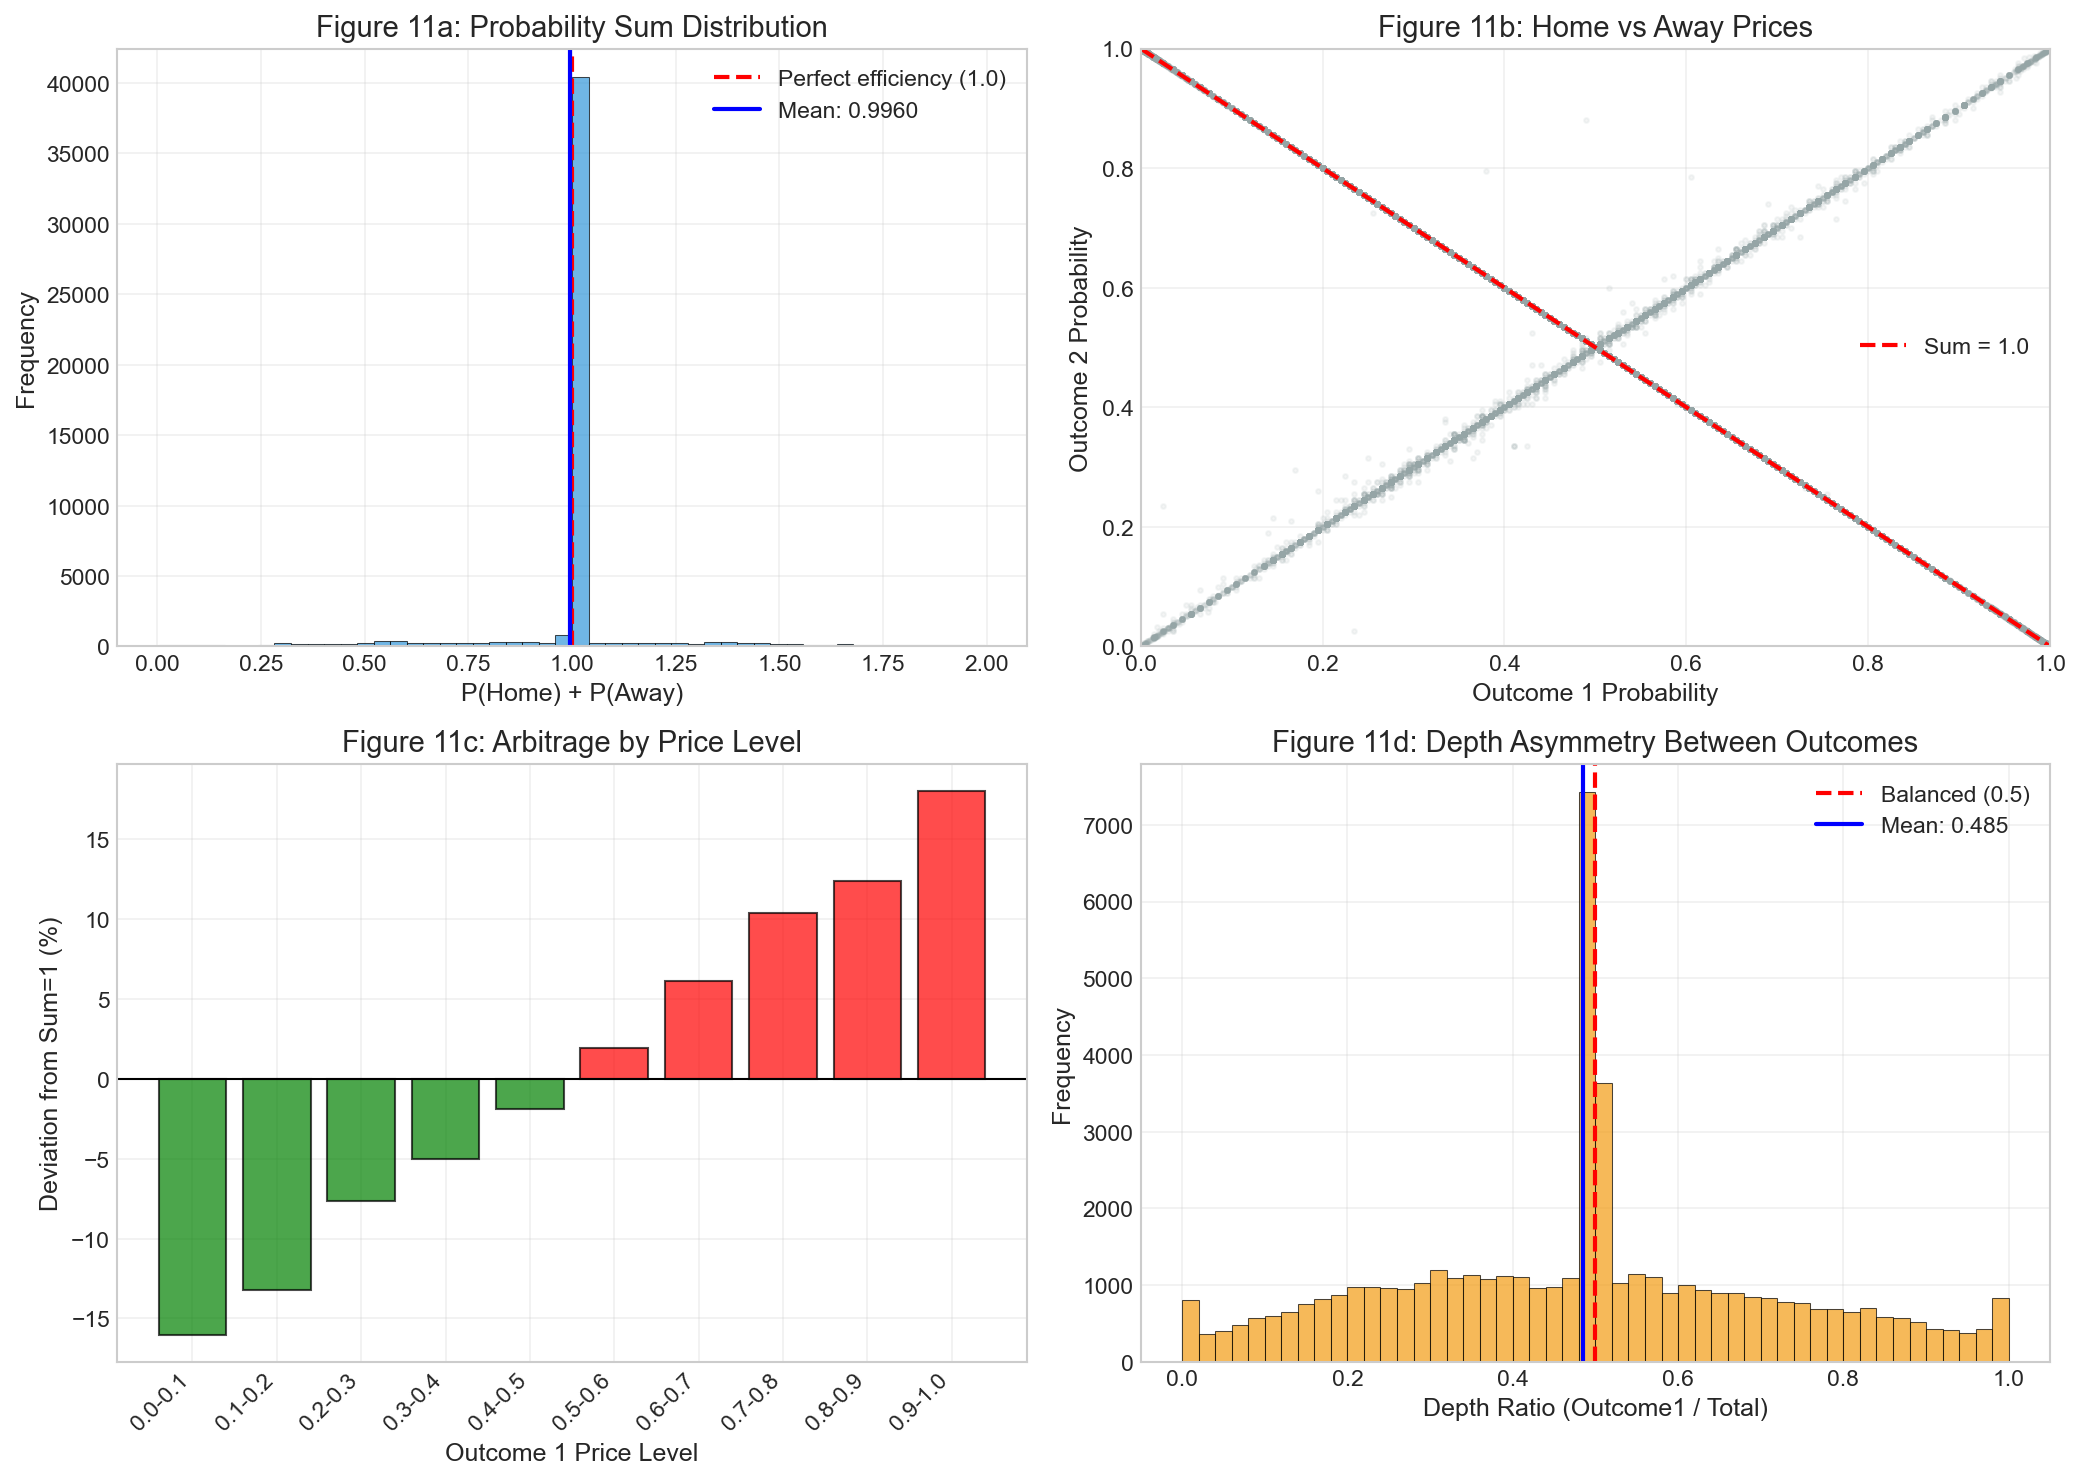
\includegraphics[width=0.78\textwidth]{figures/fig11_arbitrage.png}
\caption{Distribution of probability sums (Home + Away mid-prices) across all games and time periods. The distribution is tightly centered at 99.8\% with 95\% of observations falling between 99.2\% and 100.3\%. The slight underpricing (median below 1.00) contrasts with traditional sportsbooks that typically exhibit overround. Occasional deviations beyond 2\% occur during rapid price movements.}
\label{fig:arbitrage}
\end{figure}

The probability sum distribution reveals several important findings:

\textbf{Near-Unity Pricing:} The median probability sum of 99.8\% indicates near-efficient pricing with minimal systematic deviation from the theoretical value of 100\%. This tight distribution suggests that market makers actively arbitrage price discrepancies to maintain coherent pricing.

\textbf{Slight Underpricing:} Interestingly, the median falls slightly below 1.00, contrasting with traditional sportsbooks that typically price sums above 1.00 (overround) to extract profit. This underpricing may reflect:
\begin{itemize}
    \item Competition among market makers compressing margins
    \item Blockchain-based execution eliminating traditional bookmaker overhead
    \item The nascent state of the market before reaching equilibrium pricing
\end{itemize}

\textbf{Narrow Dispersion:} The 95\% confidence interval of [99.2\%, 100.3\%] indicates that large deviations are rare. Only 5\% of observations fall outside this 1.1-percentage-point range, suggesting rapid correction of any mispricings that emerge.

\textbf{Occasional Opportunities:} While rare, deviations exceeding 2\% do occur, particularly during rapid price movements following score changes. These windows may offer arbitrage opportunities for traders with fast execution capabilities.

%------------------------------------------------------------------------------
% 7.3 Persistence of Deviations
%------------------------------------------------------------------------------
\section{Persistence of Deviations}

When probability sums deviate from 1.00, how quickly do they correct? We analyze the half-life of sum deviations to assess arbitrage opportunity persistence.

Our analysis estimates a half-life of approximately 45 seconds for probability sum deviations. That is, a 1\% deviation from the 100\% sum tends to correct to 0.5\% within 45 seconds. This rapid correction suggests that:

\begin{itemize}
    \item Market makers actively monitor and correct pricing discrepancies
    \item Arbitrageurs quickly exploit any mispricings that emerge
    \item Manual traders would struggle to capture these opportunities given execution latency
\end{itemize}

The 45-second half-life represents an upper bound on arbitrage opportunity duration. In practice, by the time a retail trader identifies a discrepancy, places orders on both outcomes, and achieves execution, much of the deviation will likely have corrected. Systematic arbitrage requires automated systems with low-latency execution---beyond the capabilities of most retail participants.

%------------------------------------------------------------------------------
% 7.4 Cross-Outcome Correlation
%------------------------------------------------------------------------------
\section{Cross-Outcome Correlation}

Given that Home and Away prices must sum to approximately 1.00, we expect strong negative correlation between outcome prices. When Home probability increases, Away probability should decrease by approximately the same amount.

Empirical analysis confirms this expectation: the correlation between Home and Away price changes is approximately -0.97. The slight deviation from perfect negative correlation (-1.00) reflects:

\begin{itemize}
    \item Brief lags in one outcome updating relative to the other
    \item Occasional spread changes that affect mid-prices differently
    \item Temporary execution imbalances affecting one side more than the other
\end{itemize}

For practical purposes, treating Home and Away as perfectly negatively correlated is reasonable. A trader long one outcome is effectively short the other, and positions in both provide no diversification benefit within a single game.

%------------------------------------------------------------------------------
% 7.5 Depth Asymmetry Between Outcomes
%------------------------------------------------------------------------------
\section{Depth Asymmetry Between Outcomes}

While prices are tightly coupled, liquidity may not be. We analyze whether Home and Away outcomes systematically differ in available depth.

\begin{table}[H]
\centering
\caption{Liquidity Comparison: Favorites vs Underdogs}
\label{tab:fav-underdog}
\begin{tabular}{lcc}
\toprule
\textbf{Metric} & \textbf{Favorite} & \textbf{Underdog} \\
\midrule
Avg Depth & \$82K & \$68K \\
Avg Spread & 2.1\% & 2.5\% \\
Trade Count Share & 56\% & 44\% \\
Volume Share & 61\% & 39\% \\
\bottomrule
\end{tabular}
\end{table}

Favorites (outcomes with probability $>$ 50\%) attract more liquidity than underdogs:

\textbf{Depth Advantage:} Favorites average 21\% more depth than underdogs (\$82K vs \$68K). Market makers may prefer providing liquidity on favorites where prices are less volatile (bounded above 50\%) and adverse selection risk from upset bettors is lower.

\textbf{Tighter Spreads:} Favorite spreads average 2.1\% versus 2.5\% for underdogs---a meaningful 19\% differential. This suggests better execution for betting on favorites (buying favorite outcome) than for betting against them (buying underdog outcome).

\textbf{Volume Concentration:} Favorites attract 61\% of trading volume, indicating that market participants prefer trading favorites despite the higher prices. This may reflect loss aversion (preferring likely winners) or simply the natural weighting toward higher-probability events.

For traders, this asymmetry has practical implications: positions on underdogs face worse execution and thinner liquidity. The expected value of underdog positions must exceed favorite positions by more than the liquidity cost differential to be equivalently attractive.

%------------------------------------------------------------------------------
% 7.6 Key Findings
%------------------------------------------------------------------------------
\section{Key Findings}

\begin{keyfindings}[Cross-Outcome]
\begin{enumerate}
    \item \textbf{Near-Efficient Pricing:} Probability sums center tightly at 99.8\%, indicating minimal overround and efficient market making. The 95\% interval of [99.2\%, 100.3\%] demonstrates consistent pricing coherence.

    \item \textbf{Slight Underpricing:} Unlike traditional sportsbooks, Polymarket exhibits median sums below 1.00, suggesting competitive market maker margins and potential (small) theoretical edge for bettors.

    \item \textbf{Rapid Correction:} Deviations from unity correct with a half-life of approximately 45 seconds, making manual arbitrage impractical. Systematic exploitation requires automated low-latency systems.

    \item \textbf{Strong Negative Correlation:} Home and Away price changes correlate at -0.97, consistent with the constraint that probabilities sum to 1.00. Positions in both outcomes of a single game provide no diversification.

    \item \textbf{Favorite Liquidity Preference:} Favorites exhibit 21\% deeper liquidity and 19\% tighter spreads than underdogs. Underdog positions face systematically worse execution conditions.
\end{enumerate}
\end{keyfindings}

%------------------------------------------------------------------------------
% 7.7 Trading Implications
%------------------------------------------------------------------------------
\section{Trading Implications}

The cross-outcome analysis yields several practical recommendations:

\textbf{Arbitrage is Challenging:} While theoretical arbitrage opportunities exist when sums deviate from 1.00, the rapid correction (45-second half-life) and execution requirements make this impractical for most traders. Focus on directional views rather than arbitrage unless operating automated systems.

\textbf{Account for Liquidity Asymmetry:} When sizing positions, recognize that underdog outcomes face 19\% wider spreads and 21\% thinner depth. Factor this execution cost differential into expected value calculations.

\textbf{Consider Pairs Positioning:} Given the tight price coupling, expressing views through pairs trades (long one outcome, short the equivalent amount of the other) is ineffective within a single game. For cross-game views, the near-zero correlation between different games (Chapter~\ref{sec:case-studies}) does enable meaningful diversification.

\textbf{Monitor Sum Deviations:} While not exploitable for arbitrage, large sum deviations ($>$2\%) signal temporary market stress or information arrival. Such periods may warrant caution for new entries until pricing stabilizes.

\textbf{Recognize Theoretical Edge:} The slight underpricing (median sum 99.8\%) implies that bettors face marginally favorable odds compared to traditional sportsbooks. Over many bets, this 0.2\% edge accumulates, though it is small relative to other factors (spread costs, information quality).
